\begin{chapter}{Estado de los recursos}
\label{chap:estado-recursos-CITIC-VCF}

\lettrine{C}{on} el fin de contextualizar los recursos utilizados para el desarrollo del proyecto, en este capítulo se expone la situación actual de la infraestructura situada en el CITIC. Esto incluye el software que está en funcionamiento, los recursos físicos de los que se compone, y el estado actual de las herramientas que rodean a dichos recursos.

\begin{section}{Infraestructura}

    La infraestructura física donde se encuentra el servicio de virtualización, se encuentra en el edificio del CITIC de la UDC, dentro de un rack alojado en su Centro de Proceso de Datos (CPD)\cite{citicUDC}.
% La infraestructura física donde se planea desplegar el servicio de virtualización, se encuentra localizada en el edificio del CITIC de la UDC, dentro de un rack alojado en su Centro de Proceso de Datos (CPD)\cite{citicUDC}. 
\begin{subsection}{Cómputo}
    Está formada por 5 hosts Lenovo NeXtScale nx360 M5, cada uno con dos procesadores Intel Xeon E5-2650, 128 GB de memoria RAM y una tarjeta gráfica Tesla M60,  y 3 hosts Dell EMC PowerEdge R740 cada uno con dos procesadores Xeon Gold 6146, 384 GB de memoria RAM y una tarjeta gráfica Tesla P40. Todos ellos aportan flexibilidad en cuanto a que permiten escalar la infraestructura y ofrecen gran rendimiento de cómputo.
\end{subsection}
\begin{subsection}{Almacenamiento}
    El sistema de almacenamiento está colocado físicamente en la misma ubicación que los hosts pero en su abstracción lógica este es independiente y está separado de cada host. Está conformado por 13 discos duros SSD de 3.84 TB de capacidad, obteniendo así una cantidad total de casi 50 TB, pero su capacidad útil es de 34 TB ya que se utiliza la configuración de almacenamiento RAID 5 para aporta mayor integridad de los datos, mayor tolerancia a fallos y mayor ancho de banda. Los discos duros están colocados en una misma cabina formando un \textit{pool} de almacenamiento que se divide en cinco LUNs (Logical Storage Unit) de 2 TB cada una, representadas en el software de virtualización como cinco datastores, y que emplean el sistema de archivos VMFS propio de la compañía VMware, el cual optimiza el almacenamiento de máquinas virtuales.
    La configuración y gestión de este sistema se tiene que realizar al nivel de la capa física, por lo tanto si se quiere realizar un despliegue en el sistema de virtualización que requiera una configuración de almacenamiento diferente a la existente, como por ejemplo un sistema RAID con diferentes características, sería necesario modificar la configuración del sistema físico, siendo muy costoso en tiempo y riesgos. Por lo tanto, este sistema de almacenamiento no permite ajustar de forma precisa, rápida y bajo demanda la configuración de almacenamiento que un usuario requiera para sus aplicaciones.
\end{subsection}

\begin{subsection}{Red}
    El sistema de almacenamiento forma una Storage Area Network (SAN), para ello se utilizan conexiones de tipo 10 Gbit entre los hosts y las cabinas donde se encuentran los discos duros. Para soportar este tipo de conexiones, cada cabina incorpora dos controladores con conectores de tipo SFP+. Además, las cabinas de almacenamiento incorporan otros dos puertos de 1 Gbit para llevar a cabo la administración de los discos. En esta estructura se utilizan los protocolos de red Ethernet y iSCSI. Para mantener la disponibilidad del acceso al sistema de almacenamiento y aumentar la disponibilidad de de las conexiones entre hosts, cada host de ellos se conecta a dos switches \textit{trunk} para establecer rutas redundantes.
    Igual que con el sistema de almacenamiento, si se requieren realizar modificaciones sobre la red para adaptarse a los requisitos de un determinado despliegue, habría que hacerlas directamente sobre la red física. Esto puede generar problemas en la conectividad del entorno a parte de generar gran coste de tiempo.

\end{subsection}

\end{section}

\begin{section}{Software}
    \label{subsec:softwareinstalado}
    Actualmente, el software desplegado sobre la infraestructura está formado por los productos de la compañía VMware, uno de los principales proveedores de software de virtualización. Todos los componentes instalados se engloban dentro del producto \textbf{VMware vSphere}, en su versión 6.7, el cual contiene lo necesario para virtualizar la infraestructura junto con las herramientas para entregar el servicio y gestionar la infraestructura virtual. A continuación	se describen los principales componentes que tiene VMware vSphere y que están instalados en la infraestructura.
    % principal componente ya que se utiliza para virtualizar parte de la infraestructura física y proporcionar las herramientas necesarias para gestionarla, sus principales componentes internos se describen a continuación.
    \begin{figure}[h]
        \centering
        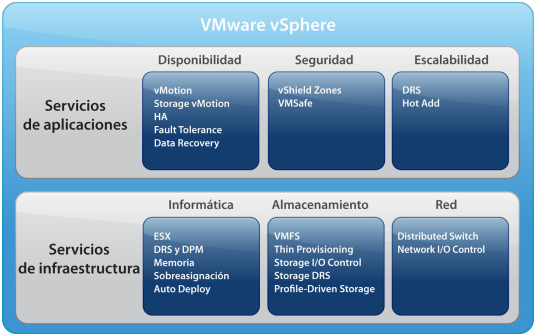
\includegraphics[width=0.75\textwidth]{imaxes/cap2recursos/contentVSphere}
        \caption{Componentes de VMware vSphere\cite{fotovSphere}}
        \label{fig:vSphere-components}
      \end{figure}
    
    En cada host está instalado el hipervisor ESXi de tipo baremetal, este se encarga de habilitar la virtualización de los recursos. Sobre los hosts se ecuentra una VM que alberga el servicio VMware vCenter Server, el cual actúa como centro de administración de todas las máquinas virtuales (VMs) y hosts que forman la infraestructura. Además, esta instancia de VMware vCenter Server contiene una instancia embebida de Platform Services Controller (PSC), punto que centraliza la autenticación en las APIs de VMware vCenter Server, actúa como servidor de licencias y contiene servicio de autenticación de usuarios llamado vCenter Single Sign-On, este último se utiliza para gestionar la autenticación de los usuarios registrados en VMware vCenter Server. El acceso e interfaz de VMware vCenter Server la proporciona el componente vSphere Web Client, una página web donde el usuario puede autenticarse y gestionar las VMs y hosts que forman el entorno y el resto de servicios de VMware vSphere. Además, incorpora vSphere Update Manager desde el cual se gestionan las actualizaciones de los componentes de VMware vSphere. Para administrar las conexiones de las VMs desplegadas en el entorno, se utiliza el componente vSphere Distributed Switch (vDS), un switch virtual donde se establecen puertos para que las VMs tengan acceso a la red y a través de los cuales se configuran las propiedades del tráfico. Finalmente, se utilizan varios servicios de gran importancia para mantener la disponibilidad de las VMs desplegadas en la infraestructura:
    
    \begin{itemize}
        \item vMotion: encarga de migrar VMs de un host a otro de forma transparente y sin detener su ejecución ni el servicio.
        
        \item vSphere High Availability (HA): encargado de recuperar el servicio de una VM que ha sufrido un fallo. Para ello, la VM es reiniciada en otro host del entorno.
        % En caso de que una VM deje de estar activa, este servicio intenta encenderla de forma automática en otro host del entorno. A diferencia de vMotion, este solo actúa en caso de que la VM o el host donde se encuentra la VM sufra un fallo y esta pase a estar no disponible. 
        
        \item vSphere Distributed Resource Scheduler (DRS): encargado de balancear la carga de trabajo entre los hosts disponibles en el entorno, migrando las VMs cuando sea necesario para maximizar el rendimiento de la infraestructura. 
        
        % vSphere DRS genera recomendaciones sobre donde se debería desplegar una máquina virtual durante su creación, utiliza vMotion para migrar las VMs y así maximizar el rendimiento o para manterner la VM activa durante tareas de mantenimiento en un host. vSphere DPM se encarga de gestionar el consumo de energía de cada host según el rendimiento actual. Sotrage DRS se encarga de balancear la carga de almacenamiento y las operaciones de lectura y escritura entre los \textit{datastores} disponibles.
        
        % \item \textbf{vSphere Fault Tolerance}: gestiona una copia de todos los archivos y discos de cada VM sincronizada con los archivos originales. Este servicio usado con vSphere HA y vSphere DRS proporciona recuperación ante fallos automática y disponibilidad continua de las VMs, sin perdida de datos y sin pérdida de las conexiones establecidas. En caso de que una VM deje de estar disponible esta se reinicia en un host diferente. Este servicio está orientado a proteger aquellas tareas que requieren un alto rendimiento o que son críticas.
    \end{itemize}
\end{section}

\begin{figure}[hp]
    \centering
    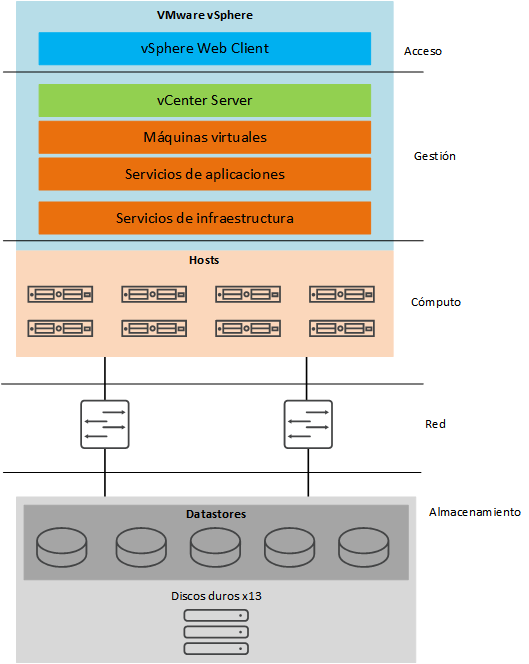
\includegraphics[width=0.6\textwidth]{imaxes/cap2recursos/recursosReal.png}
    \caption{Componentes físicos y software que forman la infraestructura actual.}
    \label{fig:infrastructure-components-production}
\end{figure}
\FloatBarrier

\begin{section}{Estado de la tecnología}
Con el desarrollo de las tecnologías web y la comercialización por parte de grandes empresas de su infraestructura, los servicios \textit{Infrastructure as a Service} (IaaS) han ganado una popularidad considerable, con ello también se han desarrollado herramientas software dedicadas a la gestión de infraestructura para la implementación de sistemas Cloud Computing. Algunas de estas son VMware Cloud Foundation (creado en 2011), OpenStack (creado en 2010) o Apache CloudStack (creado en 2012). Estos productos proveen software que permite construir una infraestructura virtualizada sobre un conjunto de recursos físicos, con el objetivo de separar la administración de la capa física de la capa virtual, y simplificar y automatizar la gestión y escalabilidad de los recursos. Proponen un modelo que persigue reducir costes de gestión de la infraestructura y aumentar la disponibilidad del servicio, es decir, aumentar la eficiencia de la infraestructura física.

Como ya se ha visto, en el mercado existen varias alternativas que se pueden utilizar para cumplir los objetivos del proyecto. Finalmente, se ha escogido el producto \textbf{VMware Cloud Foundation} (VCF) ya que se integra perfectamente con los componentes de VMware ya instalados en la infraestructura y, por lo tanto, su mantenimiento sencillo. Desplegar un producto de una compañía diferente e integrarlo con los elementos desplegados en el CITIC, podría producir problemas de compatibilidad entre versiones a largo plazo, a pesar de que este se pueda integrar con el software VMware vSphere. Utilizando los productos de un mismo proveedor se asegura el soporte del software instalado y la obtención del máximo rendimiento de cada componente.
Para poder usar este software es necesaria la adquisición de licencias. Estas se organizan por componente y por número de hosts sobre los que se va a instalar el producto. Aunque tienen un coste elevado, este producto aporta grandes beneficios.

\begin{subsection}{VMware Cloud Foundation}

    Esta solución de VMware virtualiza todas las capas de la infraestructura combinando cuatro de sus productos. Utiliza \textbf{VMware vSphere} para virtualizar y gestionar el cómputo, \textbf{VMware vSAN} para virtualizar y gestionar el almacenamiento, \textbf{VMware NSX-T} para la virtualización y gestión de la red, y \textbf{VMware vRealize Suite} para gestionar las operaciones de la infraestructura virtual como el aprovisionamiento de recursos. Todos estos servicios juntos convierten el CPD en un Software Defined Datacenter (SDDC), un entorno donde existe una infraestructura física que se abstrae en una capa virtual para separar la gestión de ambas y poder modificar la infraestructura virtual según las necesidades de los usuarios sin necesidad de modificar la configuración de la infraestructura física, y que permite a los usuarios aprovisionar recursos, construyendo así un servicio de Cloud Computing. Con esta estructura se obtienen las siguientes características:
    
\begin{itemize}

    \item Servicios software con integración nativa: ofrece un conjunto de servicios software para el almacenamiento, red, seguridad y gestión del servicio Cloud. Estos servicios se integran de forma nativa con la infraestructura minimizando las tareas de configuración y administración.

    \item Escalabilidad y elasticidad de los recursos: la capacidad de la infraestructura se puede modificar de forma sencilla gracias a la automatización del ciclo de vida de todos los elementos y al desacople entre las dos capas (la física y la virtual).

    \item Supervisión de los recursos: monitoriza los recursos con reconocimiento de aplicaciones y solución de problemas, permitiendo conocer todos los eventos que tienen lugar en la infraestructura. También permite establecer políticas de seguridad en cuanto al acceso a los recursos y la red.

    \item Aprovisionamiento automatizado: permite la obtención de recursos de forma automática incluyendo servicios de red, almacenamiento y cómputo. Los componentes de la infraestructura virtualizada se encargan de la reserva de los recursos y de todas las operaciones necesarias para llevarla acabo.

    \item Ciclo de vida automatizado: automatiza las operaciones de gestión previas, iniciales y posteriores de la plataforma para simplificar y coordinar su gestión. En estas tareas incluye el despliegue de la plataforma y su implementación, la escalabilidad de los recursos físicos y la instalación de actualizaciones para cada componente software.

\end{itemize}
\begin{figure}[h!]
    \centering
    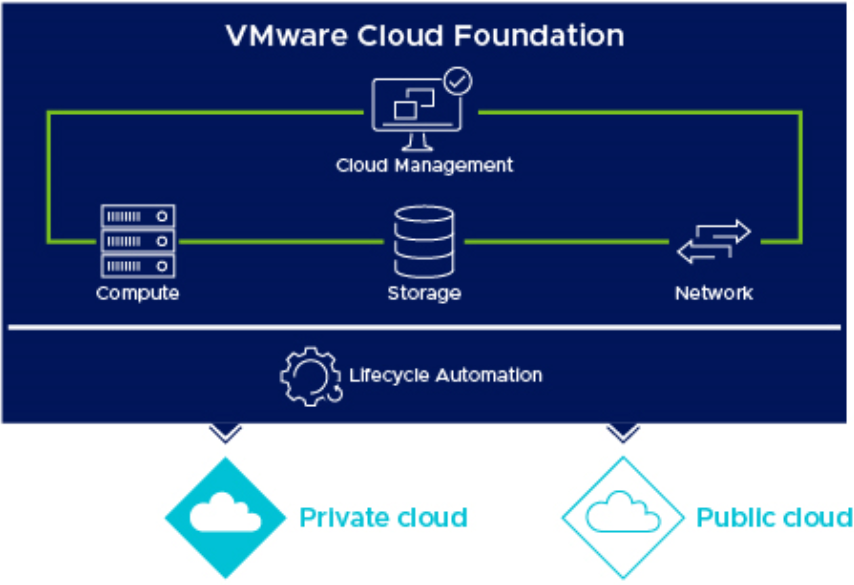
\includegraphics[width=0.6\textwidth]{imaxes/cap2recursos/overviewCF.png}
            \caption{Estructura de VMare Cloud Foundation.}
    \label{fig:Cloud-Foundation-Overview}
    \end{figure}
    \FloatBarrier
    \begin{figure}[h]
        \centering
        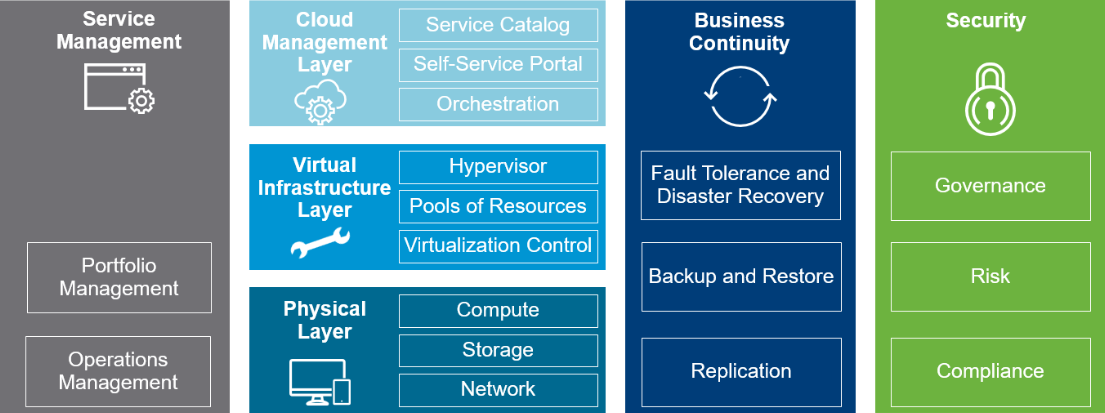
\includegraphics[width=0.8\textwidth]{imaxes/cap2recursos/SDDCoverview.png}
        \caption{Elementos de un SDDC gestionado con VMware Cloud Foundation.}
        \label{fig:layers-Sddc}
    \end{figure}
    \FloatBarrier
\end{subsection}

\begin{subsection}{Componentes de VMware Cloud Foundation}
\label{subsubsect:cfcomponents}

Ya se ha visto que VCF está formado por cuatro productos principales. En este apartado se describirán las características de esos cuatro componentes más el servicio que los coordina\footnote{Las características del componente VMware vSphere son las mismas que las descritas en el punto \ref*{subsec:softwareinstalado}}. Se utilizará la versión 4.0 de VMware Cloud Foundation lo cual implica que se implementarán las versiones\cite{componentesCloudFound} 4.0 de SDDC Manager, 7.0.0 de VMware vSphere, 7.0.0 de VMware vSAN, 3.0 de VMware NSX-T y 8.1 de VMware vRealize Suite.
\begin{figure}[h]
    \centering
        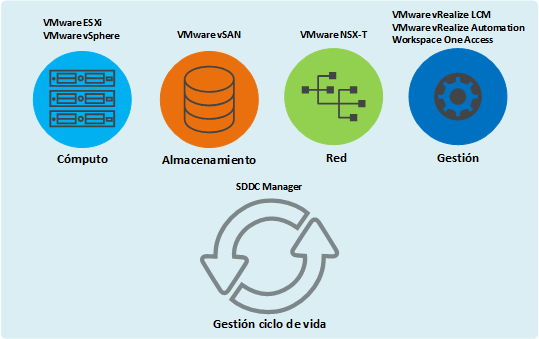
\includegraphics[width=0.6\textwidth]{imaxes/VCF-componentes/ComponentesVCF.png}
        \caption{Partes de un SDDC y componentes de VCF que las implementan.}
        \label{fig:componentes-funciones-VCF}
    \end{figure}
    \FloatBarrier
\begin{subsubsection}{SDDC Manager}
    SDDC Manager se encarga de gestionar el ciclo de vida de todos los componentes de VCF, esto incluye el despliegue de cada uno, su configuración y la obtención e instalación de actualizaciones. Centraliza la gestión de las licencias y certificados de cada componente y administra el aprovisionamiento de nuevos recursos físicos para el SDDC y los ya existentes.
\end{subsubsection}

\begin{subsubsection}{VMware vSAN}
    VMware vSAN virtualiza el almacenamiento del SDDC. Permite gestionar de forma centralizada, desde la interfaz de vSphere Web Client, el sistema de almacenamiento sin necesidad de tener que modificar la configuración física. El sistema de almacenamiento se abstrae para formar único datastore sobre el que se establecen políticas de uso y disponibilidad. El acceso por parte de cada host al datastore se realiza con el protocolo IP, a través de una subred dedicada al servicio. Con VMware vSAN, el datastore está formado por discos de almacenamiento que se organizan en grupos que se asignan a un host. Los grupos pueden tener configuración \textit{Hybrid}, que combina discos HDD y SDD, o configuración \textit{All-Flash} que solo utiliza SSD y por lo tanto tiene mayor rendimiento. Dentro de cada grupo existe un disco de caché y al menos un disco de capacidad donde se almacenan los datos persistentes\cite{operacionesVSAN}. 
    % En el modo \textit{All-Flash}\footnote{Solo se describe el modo \textit{All-Flash} porque es la configuración recomendada por VMware.} la operación de lectura se realiza directamente sobre los discos de capacidad y la operación de escritura se hace sobre el disco caché que posteriormente escribe los datos en el disco de capacidad.
    
    \begin{figure}[h]
    \centering
        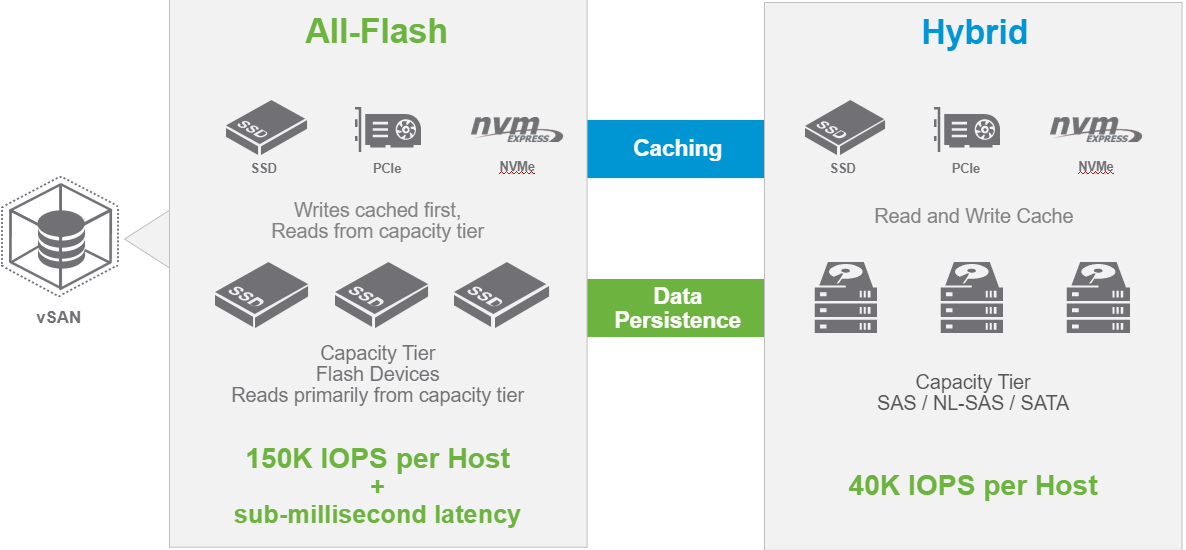
\includegraphics[width=0.6\textwidth]{imaxes/cap2recursos/rendimientoVSAN.png}
        \caption{Configuración \textit{All-Flash} y configuración \textit{Hybrid} en vSAN}
        \label{fig:performance-Hybrid-AllFlash-vSAN}
    \end{figure}
    \FloatBarrier
\end{subsubsection}

\begin{subsubsection}{VMware NSX-T}
    VMware NSX-T virtualiza la red del SDDC. Abstrae los componentes físicos de la red para generar una red virtual desacoplada de la infraestructura física, esta se configura sin modificar la red física y para ello aporta servicios de red virtualizados y la posibilidad de crear y extender subredes sobre la infraestructura. Internamente tiene tres componentes, NSX-T Manager, NSX-T Controller y NSX-T Edge. El primero, es el punto de acceso a la configuración de VMware NSX-T y el que almacena y transmite la configuración establecida, el segundo controla las redes y se encarga de informar sobre el estado y la configuración de las redes virtuales. El último componente, NSX-T Edge, proporciona servicios de red y enrutamiento a las redes virtuales. Los hosts que están integrados en VMware NSX-T se encargan de controlar el tráfico y monitorizar las conexiones que mantiene VMware NSX-T.
    % El control del tráfico y la monitorización de las conexiones se hace desde el componente \textbf{Transport Node} (TN) con la información que recibe de las instancias de NSX-T Controller. Existen dos tipos de TNs, \textbf{Hypervisor Transport Node} que son hosts con ESXi instalado y que están configurados para correr los servicios de VMware NSX-T, y \textbf{NSX-T Edge Node} que se trata de una \textit{appliance} instalada en una VM o sobre un host físico para proveer un conjunto de servicios de red centralizados para las redes virtuales de VMware NSX-T.
    \begin{figure}[h!]
        \centering
            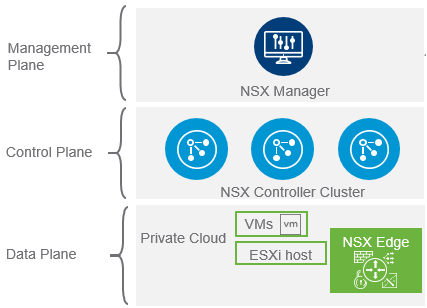
\includegraphics[width=0.6\textwidth]{imaxes/VCF-componentes/nsx-t-layers.png}
            \caption{Componentes de VMware NSX-T y capas en las que se dividen}
            \label{fig:nsx-t-components}
        \end{figure}
        \FloatBarrier
\end{subsubsection}

\begin{subsubsection}{VMware vRealize Suite}
    VMware vRealize Suite agrupa un conjunto de productos que si bien no son obligatorios para desplegar VCF, aportan funcionalidades extra que completan la formación del SDDC y del servicio Cloud. Los productos que se utilizarán en este proyecto son \textbf{vRealize Suite Lifecycle Manager} dedicado a gestionar el despliegue, actualizaciones, certificados y licencias de los productos que forman VMware vRealize, \textbf{Workspace One Access} dedicado a gestionar los usuarios y ser el punto de acceso centralizado de las aplicaciones de VMware vRealize Suite y, finalmente, \textbf{vRealize Automation} el cual permite a los usuarios del SDDC diseñar y aprovisionar un conjunto de recursos de la infraestructura según sus necesidades y de forma automatizada mientras el administrador puede limitar la cantidad de recursos que se consumen.
\end{subsubsection}

\end{subsection}

\end{section}

\end{chapter}